%!TEX root = Thesis.tex
%% ----------------------------------------------------------------
%% Author: Alex Schlosser
%%         schlosser@st.cs.uni-saarland.de
%% ---------------------------------------------------------------- 

% Set up the document
\documentclass[a4paper, 12pt, twoside, openany]{Thesis}  % Use the "Thesis" style defined in Thesis.cls
\graphicspath{{./Figures/}}  % Location of the graphics files (set up for graphics to be in PDF format)
\setchapterpath{./Chapters/}
\setappendixpath{./Appendices/}

% Include any extra LaTeX packages required
\usepackage[square, numbers, comma, sort&compress]{natbib}  % Use the "Natbib" style for the references in the Bibliography
\usepackage{verbatim}  % Needed for the "comment" environment to make LaTeX comments
\usepackage{verbatimbox}
\usepackage[usenames]{xcolor}
\usepackage{tabularx}
\usepackage{multirow}
\usepackage{wrapfig}
\usepackage{framed}
\usepackage{amssymb}
\usepackage{amsmath}
\usepackage{amsthm}
\usepackage{stmaryrd}
\usepackage{framed}
\usepackage{hyperref}
\usepackage{todonotes}
\usepackage{graphicx}
\reversemarginpar
\presetkeys{todonotes}{inline, size=\tiny, prepend, caption={TODO}}{}
\usepackage{listings}
\lstset{language=C,numbers=left}
\usepackage{longtable}
\usepackage{multicol}
\usepackage{csquotes}



%% Specify thesis parameters here
%% ----------------------------------------------------------------
\setboolean  {proposal}{false} % disables all stuff that is not needed for a proposal if set to true
\university  {Universit\"at des Saarlandes}{http://www.uni-saarland.de/}
\department  {Department of Computer Science}{http://www.cs.uni-saarland.de/}
\group       {}{}
\faculty     {juris-Stiftungsprofessur f\"ur Rechtsinformatik }{https://www.uni-saarland.de/lehrstuhl/sorge.html}
\supervisor  {Prof. Dr. Christoph Sorge}
\advisor     {Aljoscha Dietrich, M.Sc.}
\examiner    {Prof. Dr. Christoph Sorge}
\secondexaminer {Dr. Mario Fritz}
\degree      {Master of Science}
\thesiskind  {Master Thesis}
\authors     {Gautam Sawala}
\thesistitle {Privacy implications of wearable devices - identification of short movies utilizing physiological data}
\date        {\today}
%\subject     {}
%\keywords    {}
%% ----------------------------------------------------------------

% If this is a proposal prepend 'Proposal for a' to thesiskind
\doifproposal{
	\let\thesisnameproposal\thesisname
	\thesiskind{Proposal for a \thesisnameproposal}
}

% Enable git revision parsing (Note: you need to enable shell-excape and pipe support for this feature to work)
%\revision{\input{|"git rev-parse HEAD | cut -c 1-8"}}

\begin{document}
\frontmatter	  % Begin Roman style (i, ii, iii, iv...) page numbering

%% Title Page
%% ----------------------------------------------------------------
\maketitle

%% Declaration Page required for the Thesis, your institution may give you a different text to place here
%% ----------------------------------------------------------------
\doifnotproposal{
\begin{declaration}
  \begin{center}
    \bf \large
    Eidesstattliche Erkl\"{a}rung
  \end{center}
  Ich erkl\"{a}re hiermit an Eides Statt,
  dass ich die vorliegende Arbeit selbstst\"{a}ndig verfasst und keine
  anderen als die angegebenen Quellen und Hilfsmittel verwendet habe.

  \begin{center}
    \bf \large
    Statement in Lieu of an Oath
  \end{center}
  I hereby confirm that I have written this thesis on my own and 
  that I have not used any other media or materials than the ones
  referred to in this thesis.

  \vfill
  \begin{center}
    \bf \large
    Einverst\"{a}ndniserkl\"{a}rung
  \end{center}
  Ich bin damit einverstanden, dass meine (bestandene) Arbeit in beiden 
  Versionen in die Bibliothek der Informatik aufgenommen und damit 
  ver\"{o}ffentlicht wird. 

  \begin{center}
    \bf \large
    Declaration of Consent
  \end{center}
  I agree to make both versions of my thesis (with a passing grade) 
  accessible to the public by having them added to the library of the
  Computer Science Department.

  \vfill
  \vfill
   
  Datum/Date:\\
  \rule[1em]{25em}{0.5pt}  % This prints a line to write the date

  Unterschrift/Signature:\\
  \rule[1em]{25em}{0.5pt}  % This prints a line for the signature
   
\end{declaration}
  \cleardoublepage  % Declaration ended, now start a new page
}

%% The Abstract Page
%% ----------------------------------------------------------------
\begin{abstract}
	\input{\chapterpath Abstract}
\end{abstract}

\doifnotproposal{

%% The Acknowledgements page, for thanking everyone
%% ----------------------------------------------------------------
\begin{acknowledgements}

Thx Mom+Dad $<3$

\end{acknowledgements}
\cleardoublepage
}

%% Table of Contents
%% ----------------------------------------------------------------

\tableofcontents
\clearpage

%% The Dedication page
%% ----------------------------------------------------------------
\doifnotproposal{
  \thispagestyle{empty}  % Page style needs to be empty for this page
  \dedicatory{Dedicated to WHATEVER.}
}

\mainmatter	  % Begin normal, numeric (1,2,3...) page numbering

%% Chapters
%% ----------------------------------------------------------------
% Include the chapters of the thesis, as separate files (careful of case-sensitivity and spaces in filenames)
% Capitalized chaptertitles generally look better

\loadchapter{Introduction}{Introduction}
\loadchapter{Motivation}{Motivation}
\loadchapter{Terminology}{Terminology and Significance}
\loadchapter{Related_Work}{Related Work}
\loadchapter{Data_Collection}{Data Collection}
\loadchapter{Evaluation}{Evaluation and Results}
\loadchapter{DiscussionConclusion}{Discussion and Conclusion}



%% Appendices
%% ----------------------------------------------------------------
\appendix

%%!TEX root = ../Thesis.tex
\newpage
\label{appendix_consent}
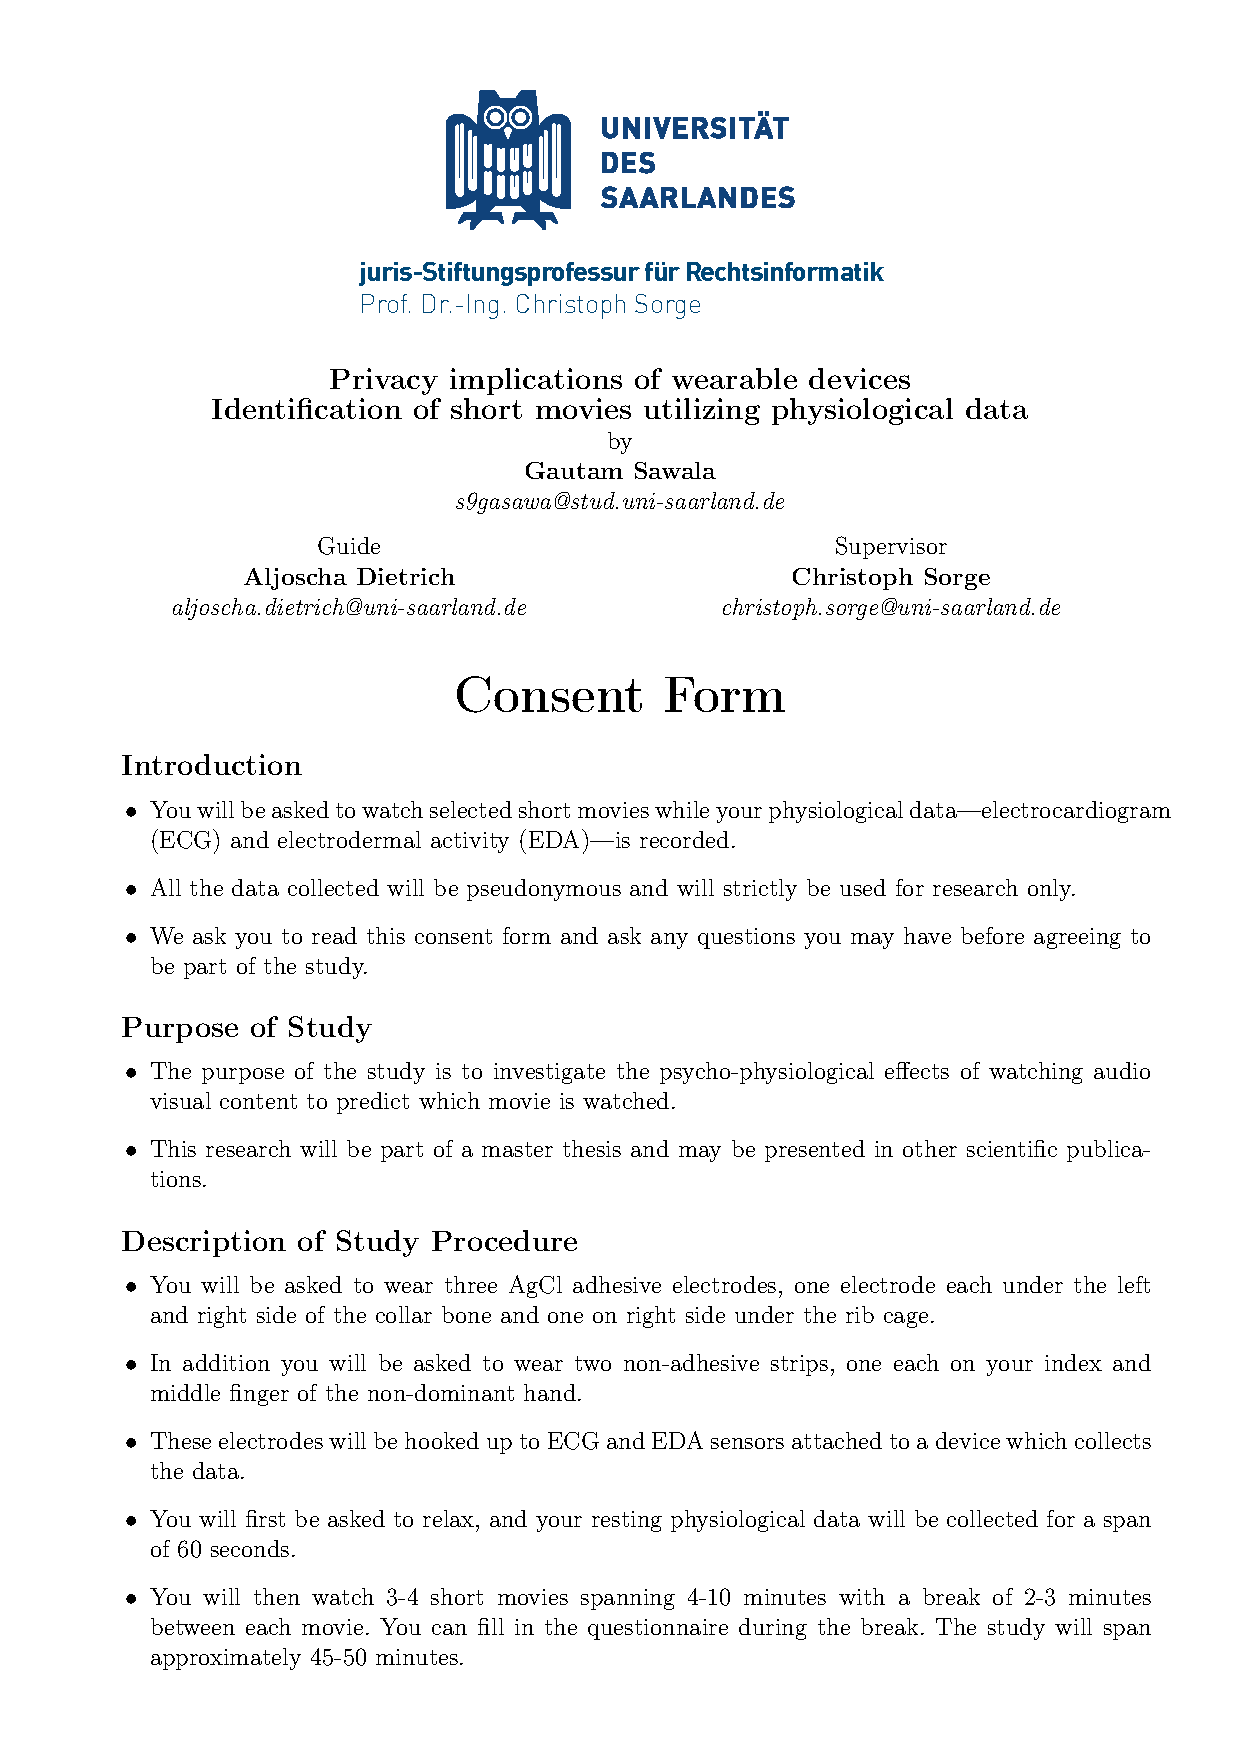
\includegraphics[page=1,width=150mm]{pdf/consent.pdf}
\newpage
\includegraphics[page=2,width=150mm]{pdf/consent.pdf}
	% Appendix Title

%%!TEX root = ../Thesis.tex
\begin{figure}
    \centering
    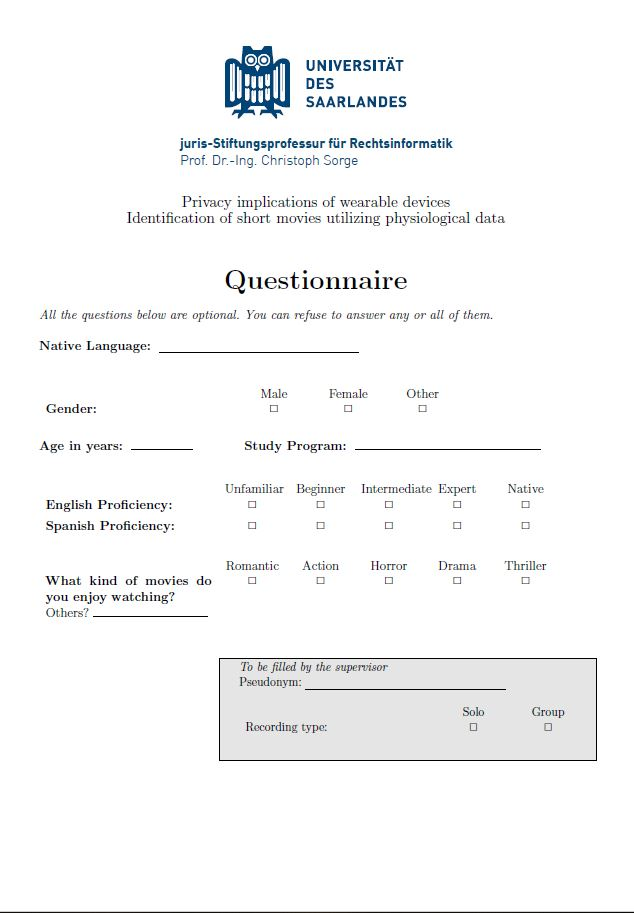
\includegraphics[width=150mm]{question_01.JPG}
    \label{fig:eda_filtering}
\end{figure}
\begin{figure}
    \centering
    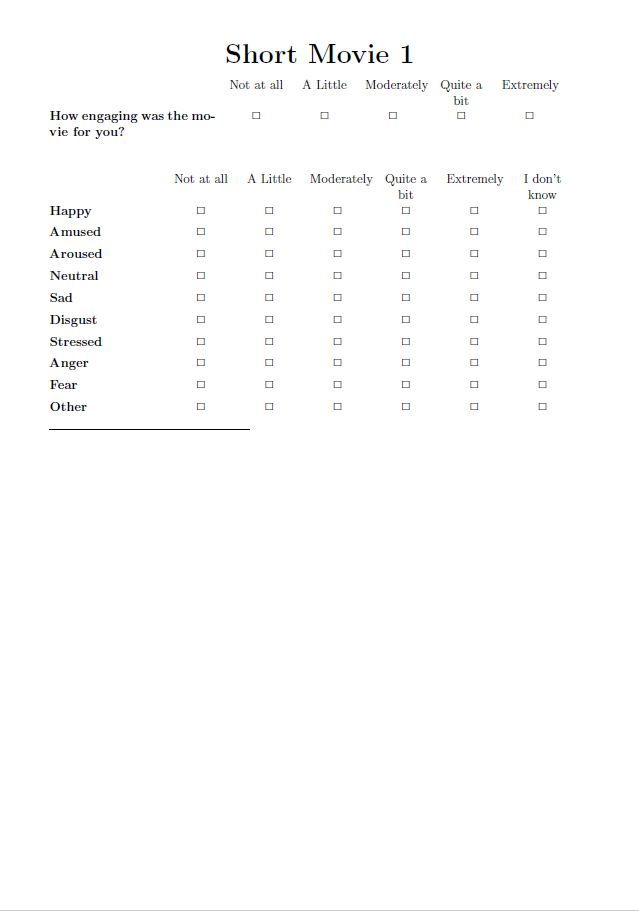
\includegraphics[width=150mm]{question_02.JPG}
    \label{fig:eda_filtering}
\end{figure}
\begin{figure}
    \centering
    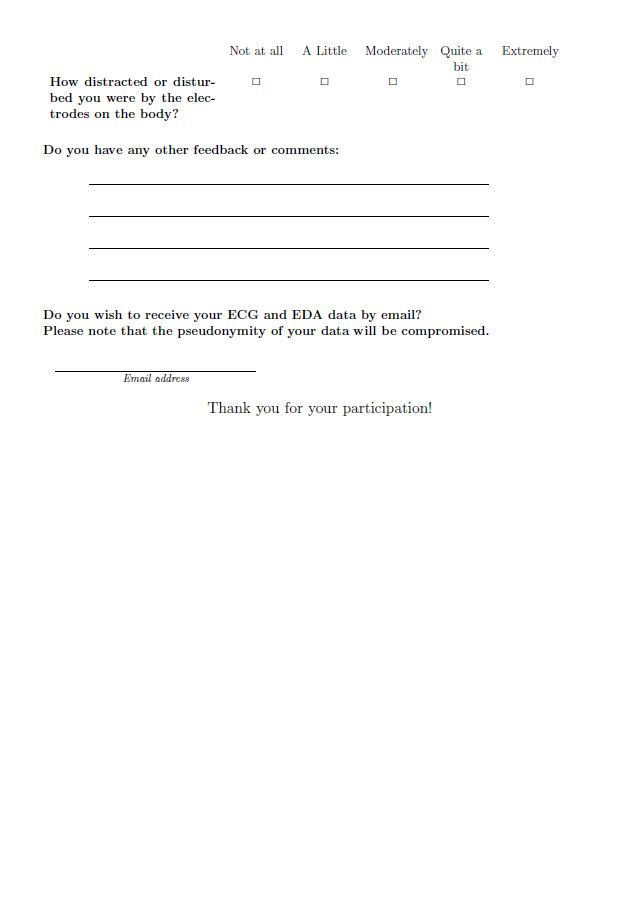
\includegraphics[width=150mm]{question_03.JPG}
    \label{fig:eda_filtering}
\end{figure} % Appendix Title

%%!TEX root = ../Thesis.tex
\newpage
\label{assessment}
\begin{figure}
\centering
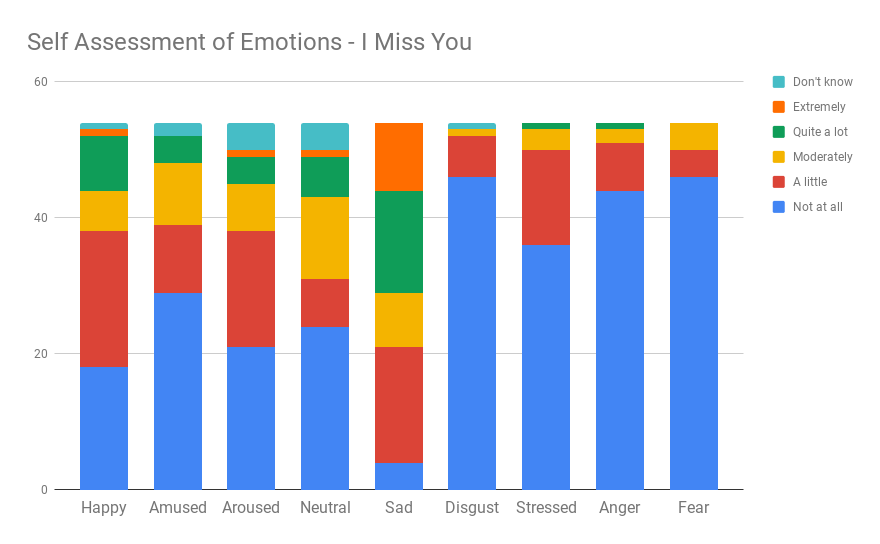
\includegraphics[width=140mm]{Figures/i_miss_you.png}
\caption{Self assessment of emotions by subjects for I Miss You movie.}
\label{fig:i_miss_you}
\end{figure}

\begin{figure}
\centering
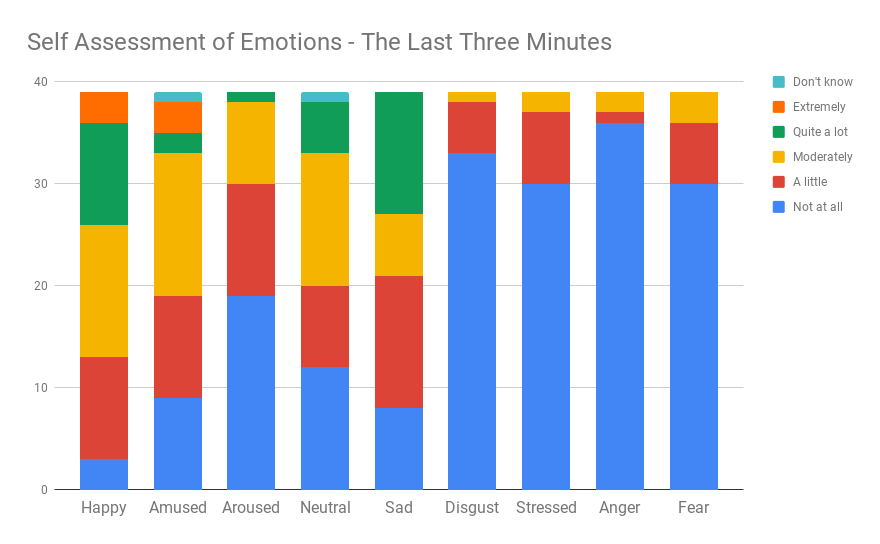
\includegraphics[width=140mm]{Figures/the_last_three_minutes.png}
\caption{Self assessment of emotions by subjects for The Last Three Minutes movie.}
\label{fig:the_last_three_minutes}
\end{figure}

\begin{figure}
\centering
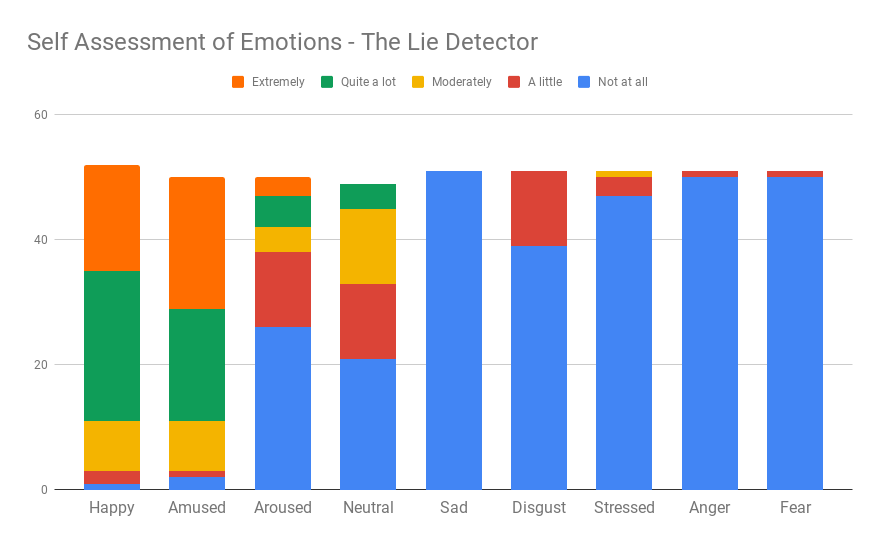
\includegraphics[width=140mm]{Figures/the_lie_detector.png}
\caption{Self assessment of emotions by subjects for The Lie Detector movie.}
\label{fig:the_lie_detector}
\end{figure}

\begin{figure}
\centering
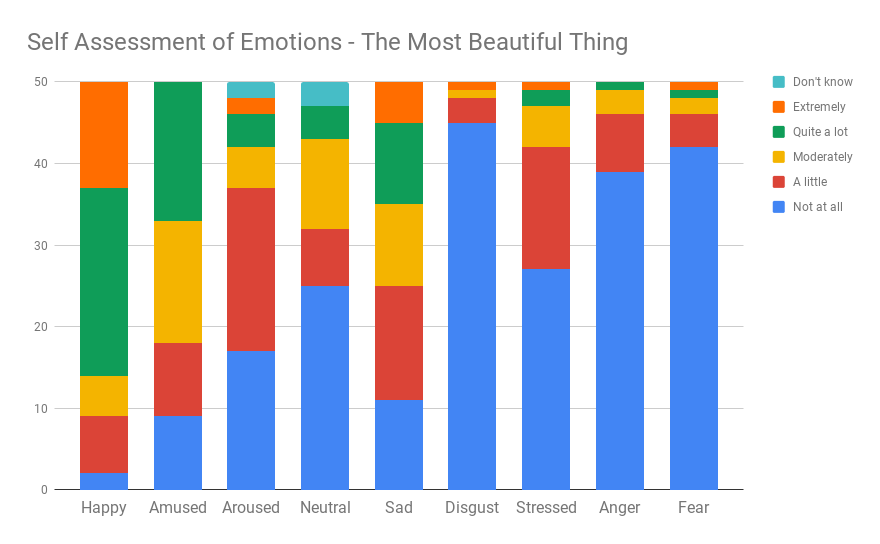
\includegraphics[width=140mm]{Figures/the_most_beautiful_thing.png}
\caption{Self assessment of emotions by subjects for The Most Beautiful Thing movie.}
\label{fig:the_most_beautiful_thing}
\end{figure}

\begin{figure}
\centering
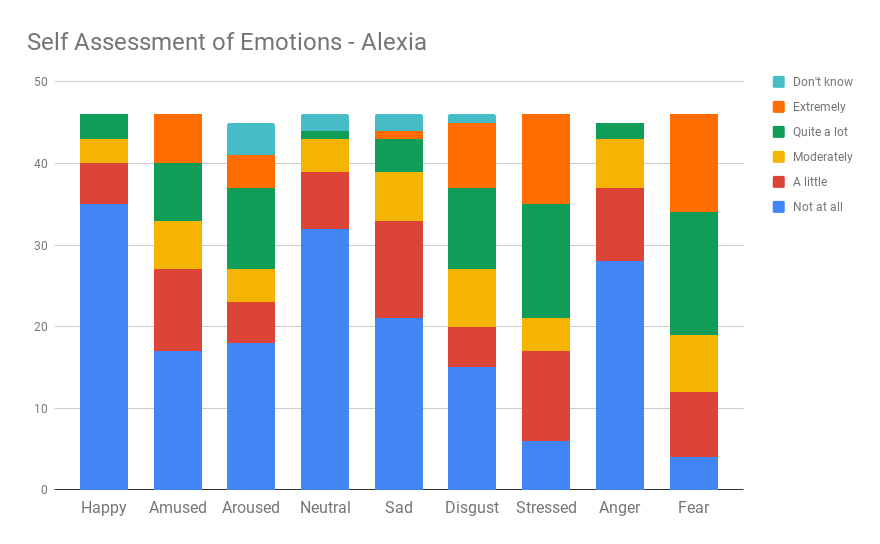
\includegraphics[width=140mm]{Figures/alexia.png}
\caption{Self assessment of emotions by subjects for Alexia movie.}
\label{fig:alexia}
\end{figure}

\begin{figure}
\centering
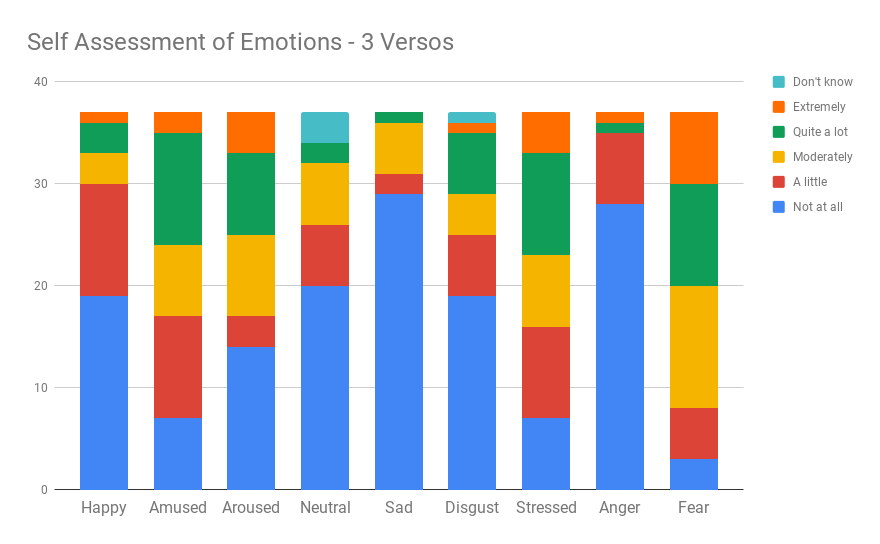
\includegraphics[width=140mm]{Figures/3_versos.png}
\caption{Self assessment of emotions by subjects for 3 Versos movie.}
\label{fig:3_versos}
\end{figure}

\begin{figure}
\centering
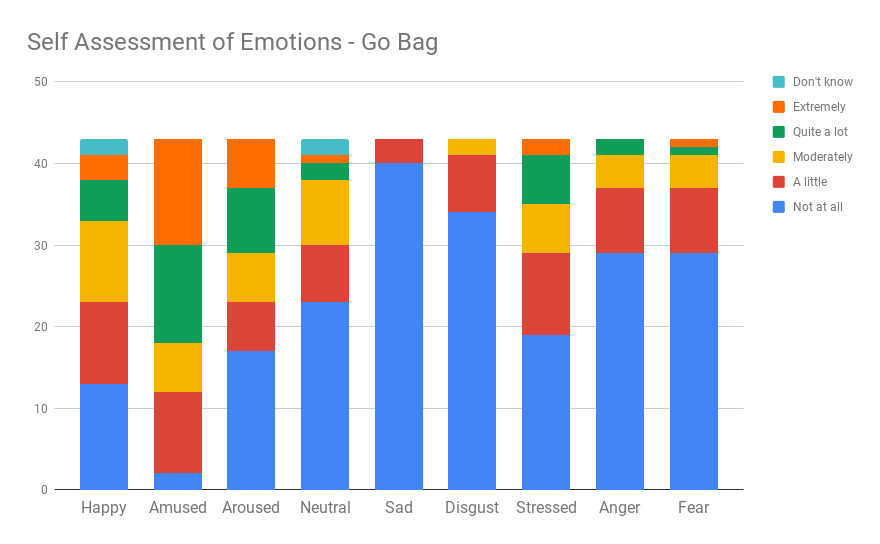
\includegraphics[width=140mm]{Figures/go_bag.png}
\caption{Self assessment of emotions by subjects for Go Bag movie.}
\label{fig:go_bag}
\end{figure} % Appendix Title


\backmatter

%% Lists of figures and tables
%% ----------------------------------------------------------------
\doifnotproposal{
	\lhead{\emph{List of Figures}}
	\addtotoc{List of Figures}
	\listoffigures
	\clearpage

  	\addtotoc{List of Tables}
  	\lhead{\emph{List of Tables}}
	\listoftables
	\clearpage
}

%% Bibliography
%% ----------------------------------------------------------------
\label{Bibliography}
\addtotoc{Bibliography}
\lhead{\emph{Bibliography}}  % Change the left side page header to "Bibliography"
\bibliographystyle{unsrtnat}  % Use the "unsrtnat" BibTeX style for formatting the Bibliography
\bibliography{Bibliography}  % The references (bibliography) information are stored in the file named "Bibliography.bib"

\beginappendix %Begins the appendix
\appendix
\loadchapter{AppendixA}{Consent Form}
%%\loadappendix{Appendix}{Consent Form}
\appendix
\loadchapter{AppendixB}{Questionnaire}
\end{document}  % The End
